%-----------------------------------------------------------------------------------------------------------------
\chapter{Estado da Arte}
\label{Ch:EstadoDaArte}
%-------------------------------------------------------------------------------------------------------------
% Last edited here
\hspace{1cm}Nas \textit{small and medium enterprises} (SME) do setor das Tecnologias da informação (IT), uma alteração ao software nas fases tardias de desenvolvimento é uma aposta que -- no cenário mais pessimista -- pode colocar tudo em jogo. Tendo em conta que as SME são a espinha dorsal da economia Europeia, surge um desafio do seu lado para dar resposta às necessidades dos consumidores de forma rápida e conectada \cite{dunne2015social}. É necessário apresentar uma solução de melhoria contínua para o típico consumidor que está a amadurecer tecnologicamente e exige cada vez mais qualidade dos serviços e produtos que consome.

\section{Hábitos comportamentais}

\hspace{1cm}Quando se produz software, para dar resposta aos requisitos dos clientes, os longos períodos de espera entre \textit{releases} são um risco que pode levar à perda de quota de mercado. A recolha e análise de feedback em tempo útil, sobre se o software -- em desenvolvimento -- vai de encontro aos requisitos de grandes números de utilizadores, é praticamente impossível. Com a introdução de metodologias \textit{Agile}, o software a ser desenvolvido vai sendo testado muito mais cedo no processo de desenvolvimento pelo cliente final e assim é possível analisar o seu comportamento e recolher feedback sobre a sua adequação em termos de solução. Assim sendo, a redução do \textit{time-to-market} e dos \textit{feedback-loops} vai permitir diminuir a discrepância entre aquilo que os \textit{Product Owners} (PO's), \textit{developers} e utilizadores entendem como boas ou más propostas de valor  \cite{raud2016caseStudy}. Evidentemente, nenhuma organização, \textit{developer} ou cliente quer investir tempo e recursos financeiros no desenvolvimento do produto errado. Para além disso, é reconhecido pela indústria de software que os ciclos de \textit{releases} podem ser períodos tensos e frustrantes. Estes sentimentos são conduzidos pelo risco de ocorrerem falhas associadas ao processo de publicação de software para produção. Em projetos de software onde as \textit{releases} são processos manuais intensivos, os ambientes que albergam o software são construídos individualmente, normalmente pelas equipas de operações sendo que, em muitos casos, a equipa de desenvolvimento também intervém nos processos de \textit{deployment}. O software de terceiros que a aplicação necessita para funcionar é instalado, os artefactos das aplicações são copiados para o(s) ambiente(s) de produção e a informação sobre a configuração é copiada ou criada através da consola de administração dos \textit{web servers}, \textit{application servers} ou componentes isolados que integram o sistema. Só depois, os dados das referências são copiados e, finalmente, a aplicação é executada serviço a serviço, componente a componente. Os sentimentos de tensão e nervosismo estão presentes por razões claras. Citando os autores \shortciteA{farley2010contdel}: \textit{``Muitas fases podem correr mal neste processo. Se cada um dos passos não for executado de forma perfeita, a aplicação não vai ser executada corretamente. E, neste ponto, pode não ser claro -- de todo -- qual é o erro, ou qual foi o passo que falhou.''}

\hspace{1cm}Esta é a principal razão pela qual, com o decorrer do tempo, os \textit{deployments} devem tender para ser o mais automatizados possível, não só pela redução do tempo ocupado pelo processo, mas também pelo aumento da resiliência do sistema e pela sucessiva eliminação de falhas provocadas pelo fator humano. Quando não são totalmente ou maioritariamente automatizados, os erros podem (potencialmente) ocorrer sempre que um \textit{deploy} manual for feito. A solução não passa só por perceber se os erros são ou não significantes. Mesmo com excelentes testes de \textit{deployment} os bugs podem ser difíceis de encontrar. Quando os \textit{deployments} não são automáticos o risco de falha aumenta e perde-se a capacidade de serem repetidos de maneira exata -- que leva a desperdícios de tempo -- e, em alguns casos, resulta na impossibilidade de identificar o problema por se desconhecer o processo exato. Um \textit{deployment} manual é uma tarefa complexa, que consome imenso tempo e envolve a colaboração de várias pessoas. É natural que, a cada passo, a documentação criada esteja incompleta ou desatualizada. Por outro lado, em \textit{deploys} automáticos, os \textit{scripts} desenvolvidos podem servir de documentação e vão estar sempre o mais atualizados possível. Se fosse de outra forma, o \textit{deployment} não iria ser concluído com sucesso \cite{farley2010contdel}. 

\section{Práticas correntes}

\hspace{1cm}Ainda de acordo com os autores \shortciteA{farley2010contdel}, integração contínua (CI -- \textit{continous integration}) permite-nos manter a aplicação funcional depois de iteração de novo código e o seu complemento, entrega contínua (CD -- \textit{continuous delivery/deployment}) dá-nos a possibilidade de lançarmos versões novas e funcionais do software, várias vezes por dia. Isto significa que o código produzido e colocado no repositório -- no \textit{branch} principal -- está com qualidade para permitir que as aplicações sejam entregues em qualquer instante. Uma \textit{delivery pipeline} (DP) compreende tanto \textit{continuous integration} de código -- numa primeira fase -- como \textit{continuous delivery} e \textit{deployment} de software para ambientes de teste ou de produção.

\subsection{Integração Contínua}

\hspace{1cm}Uma das primeiras propostas de integração contínua foi feita por \shortciteA{beck2000extreme} como uma das muitas práticas integrantes de \textit{Extreme Programming} (http://www.extremeprogramming.org/). Integração contínua é o primeiro passo na implementação de uma DP e, apesar de não depender do tamanho da equipa de desenvolvimento de software, torna-se especialmente útil com o aumento do número de \textit{developers} a colaborar em conjunto. O objetivo desta mudança é a união de todos os códigos produzidos por eles, existindo um ponto central com o código final e a garantia de que estes módulos se integram devidamente. Com a existência deste ponto central, com o código completo, é possível a implementação de processos automáticos que permitam validar desde processos básicos, como se o código é compilável sem erros, até a processos mais avançados, como testar se o código em si funciona como é esperado. Os resultados destes processos podem permitir ou impedir que o processo continue para fase seguinte. É dada prioridade às \textit{builds} bem sucedidas e ao desenvolvimento de forma que nos permita integrar código sem quebrar o fluxo, ou seja, é recomendado que cada \textit{developer} valide previamente o processo de junção do código antes de o partilhar com os restantes colegas, de forma a evitar que estes fiquem impedidos de trabalhar devido a falhas existentes. Esta mudança é um desafio cultural para equipas de desenvolvimento habituadas a métodos tradicionais. Segundo \shortciteA{startingscaling}: \textit{``Até ser feito, não se consegue imaginar que alguma vez vá funcionar mas, assim que é feito desta forma, não se imagina trabalhar de outra forma. O desafio é assegurarmo-nos que as mudanças culturais ocorrem e que as equipas estão a abraçar esta nova forma de trabalhar.''}

\hspace{1cm}Esta é uma prática que requer que os \textit{developers} façam partilhas (\textit{commit}) dos seus códigos para um sistema de controlo de versões (VCS) pelo menos uma vez por dia, como os autores \shortciteA{fowler2006continuous} sugerem. Depois do \textit{commit} das mudanças no \textbf{VCS}, um orquestrador de processos inicia a \textit{pipeline} de integração contínua para integrar as mudanças do código recebido com o resto do código, é disparado um \textit{trigger} e é feita uma \textit{build} que executa análise estática primeiro, para depois compilar e executar todos os testes unitários disponíveis \cite{raud2016caseStudy}. Um exemplo de uma \textit{pipeline} de integração e entrega contínua (CI/CD) pode ser visto na figura \ref{Fig:Fig2}. 

\hspace{1cm}Se, em qualquer fase da \textit{pipeline}, existir uma falha durante o processo de \textit{build} o seu estado é considerado como \textit{failed}. Em todo o caso, o \textit{developer} é informado acerca do resultado, quer através de feedback sob forma de notificação nos canais de comunicação da empresa (Slack/SMS, ou e-mail para notificações em tempo real), quer através do sistema de visualização integrado no processo de desenvolvimento. 

\begin{figure}
\centering
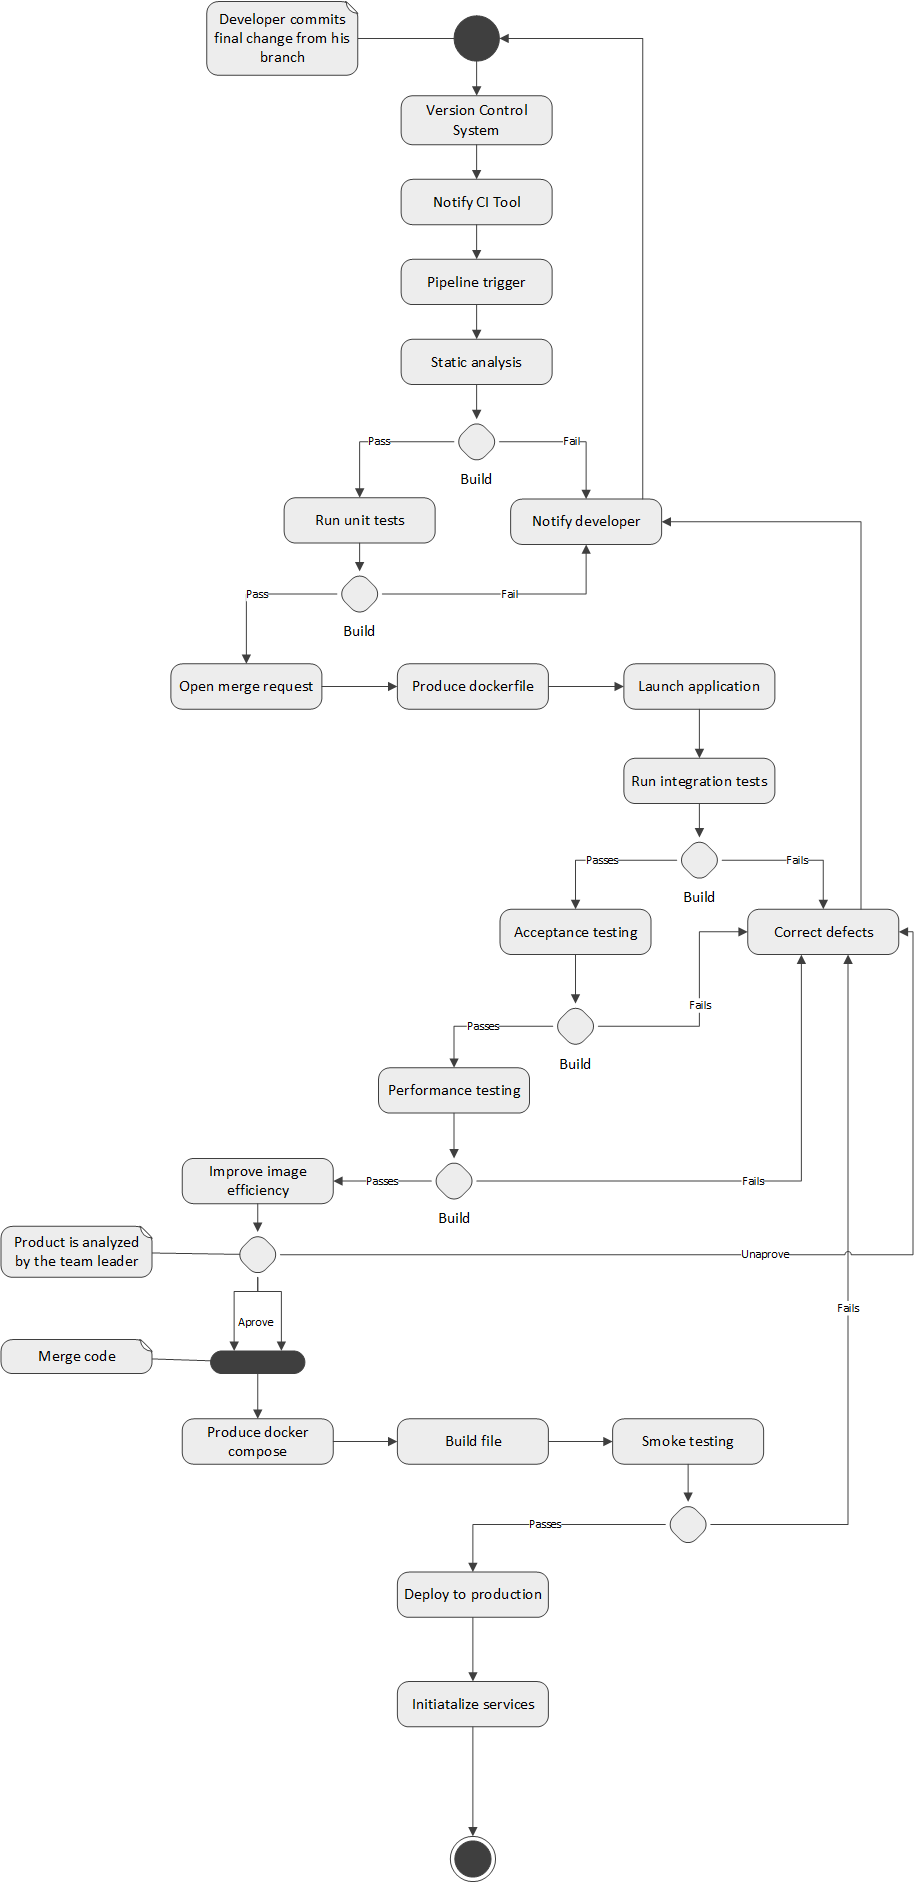
\includegraphics[width=0.7\linewidth]{Cap2/Pipeline_Workflow_UML.png}
\label{Fig:Fig2}
\end{figure}

\hspace{1cm}Quando existe mais do que um \textit{developer}, ou naqueles casos em que se está a desenvolver uma aplicação modular, a possibilidade de introdução de \textit{branches} -- uma espécie de réplica da linha principal -- permite que seja realizado desenvolvimento de uma determinada funcionalidade de forma independente e facilita que o código seja depois unido à linha principal sem que outros programadores sejam forçados a aguardar a sua conclusão \cite{farley2010contdel}.

\hspace{1cm}Fundamentalmente, a integração contínua exige a capacidade de manter a aplicação funcional depois de iterar novo código. Por forma a aumentar a qualidade do desenvolvimento do software, existem algumas abordagens ao desenvolvimento que podem ser úteis para aumentar a qualidade do produto final. Uma delas é o Desenvolvimento Orientado a Testes (\textit{TDD -- Test Driven Development}) proposto por \shortciteA{BeckTDD2002}, que propõe o desenvolvimento orientado a testes como sendo a ideia de que, quando estamos a desenvolver novas funcionalidades ou corrigimos erros, os \textit{developers} criam primeiro um teste que é uma especificação executável para o comportamento esperado do código a ser escrito. Estes testes motivam o \textit{design} das aplicações servindo de testes de regressão e, simultâneamente, de documentação de código e do comportamento esperado da aplicação \cite{farley2010contdel}.

\subsection{Entrega Contínua}

\hspace{1cm}Entrega contínua exige que sejamos capazes de fazer \textit{deploys} da aplicação a qualquer momento tanto para ambientes de teste como para ambientes de produção \cite{farley2010contdel}. Uma das técnicas chave para mantermos as aplicações publicáveis a qualquer instante -- mesmo apesar das mudanças constantes -- é a modelação dos componentes da aplicação e utilização de interfaces de comunicação. Imagine-se um componente como um grande bloco de código dentro de uma aplicação (com uma Web API bem documentada) que pode eventualmente ser trocada por outra implementação desde que respeite a interface definida. Um sistema de software baseado em componentes é distinguido pelo facto de que a sua base de código está dividida em pedaços discretos que providenciam comportamento sob forma de interações limitadas, através dessas interfaces bem definidas, com outros componentes \cite{farley2010contdel}.

\hspace{1cm}A utilização de \textit{pipelines} de integração contínua em produção e desenvolvimento de software, pode poupar muitas horas de trabalho. Partindo do  código-fonte no \textbf{VCS}, construir a aplicação, executar análise estática, testes unitários, empacotar e publicar a aplicação para um repositório remoto, são processos que consomem algum tempo. Este tempo aumenta com a complexidade e tamanho da aplicação e, por vezes, é tempo que podia ser investido no desenvolvimento de uma funcionalidade em vez de desperdiçado na execução repetitiva de um conjunto de instruções. 

\hspace{1cm}De qualquer das formas, a automatização deste processo deve ser planeada de acordo com o tamanho e modularidade de cada aplicação. Para aplicações mais complexas, podem ser necessárias várias imagens para que a aplicação seja executada. Podem existir inúmeros \textit{deployments} em múltiplos locais -- dependendo da quantidade de fases existentes -- e pode ser necessário ajustar o número de \textit{deployments} dependendo da infraestrutura que a organização tem ao seu dispor.

\hspace{1cm}Imagine-se um contexto em que um projeto exige a integração de código de cinco \textit{developers} diferentes, sendo cada um responsável por funções diferentes dentro da \textit{stack} de tecnologias a usar (BD, backend, frontend, etc). Se o \textit{Product Owner} dá preferência à utilização das práticas de \textit{DevOps} com o projeto em fase final, o projeto vai precisar não só de um ajuste em termos de estrutura organizacional, mas também de uma revisão geral de todos os processos. Neste caso em particular, a equipa está a desenvolver uma plataforma de \textit{e-commerce} e as várias arquiteturas do sistema estão fechadas, sendo apenas necessárias pequenas correções em alguns serviços que a compõem. Aqui, evidentemente, dado o grau de complexidade do sistema em desenvolvimento e o tempo investido na sua modelação -- não só em termos macro (plataforma), como também em termos micro (serviços) -- é mais vantajoso manter as práticas correntes e continuar com o mesmo método de trabalho. Nem sequer se coloca em cima da mesa outro conjunto de fatores como por exemplo a barreira cultural da resistência à mudança. O projeto iria precisar de uma revisão geral tão extensa que todo o tempo de todos os integrantes da equipa teria de ser investido na revisão de metodologias de trabalho. Isto representaria largos períodos de tempo que, obviamente, são cruciais para a finalização dos serviços que compõem a plataforma no imediato e que não podem sequer ser considerados em termos monetários.

\hspace{1cm}Noutro contexto, dispõe-se exatamente da mesma equipa de \textit{developers} a trabalhar no desenvolvimento de uma aplicação web de submissão de currículos. E um dos requisitos do \textit{business}, com o projeto em fase de arranque, indica que o desenvolvimento será feito mediante as práticas da cultura \textit{DevOps}. Neste caso, a equipa não tem qualquer tipo de ideia de qual será o alinhamento -- em termos de arquitetura -- do sistema. Aqui, contrariamente ao exemplo anterior, não tendo ainda sido investido tempo na modelação do sistema nem no seu planeamento, faz sentido a adoção das práticas de \textit{DevOps} uma vez que a mudança na cultura de trabalho será feita a partir do começo do projeto, abrindo-se espaço a um processo gradual de adaptação.

\hspace{1cm}A cultura \textit{DevOps} é portanto um complemento fundamental ao desenvolvimento \textit{Agile} e os benefícios das suas práticas são promissores. A implementação deste tipo de práticas traz imensas vantagens para o desenvolvimento de software em equipa. Em contrapartida, quanto mais tardia for a mudança para este conjunto de normas ou práticas diárias, mais difícil será a adaptação. A filosofia \textit{Agile}, por si só, é muita das vezes considerada insuficiente ou ineficaz na gestão de projetos de desenvolvimento de software. Daí ser comum encontrar outros conjuntos de técnicas e estratégias de gestão aliados a esta filosofia, como é o caso do \textit{Scrum} (https://www.atlassian.com/agile/scrum) para gestão do trabalho de vários elementos e do \textit{Kanban} (https://www.atlassian.com/agile/kanban) para representação visual do fluxo de trabalho.

\hspace{1cm}Considerando que as metodologias de gestão e planeamento devem contabilizar vários fatores internos e externos à equipa responsável pela execução do projeto, desde as políticas da internas da empresa até ao contexto do negócio, é importante ter em conta que a produção deste protótipo tem como objetivo ir de encontro à prestação de serviços \textit{business-to-business} (B2B).

\hspace{1cm}Naquilo que à prestação de serviços diz respeito, é o \textit{Information Technology Infrastructure Libary} (ITIL) conhecido como um dos conjuntos detalhados de boas práticas que se concentra no alinhamento de serviços de IT com as necessidades dos negócios. Resumidamente, o \textbf{ITIL} baseia-se em quatro disciplinas -- \textit{service request}, \textit{incident}, \textit{change} e \textit{problem}.

\hspace{1cm}O \textbf{ITIL} atua sobre três pontos cruciais de \textit{IT Service Management} (ITSM). São eles os processos, a comunicação e a transparência. Este conjunto de práticas \textit{post-deployment} atua sobre \textbf{processos} pouco (ou nada) definidos e implementados com as ferramentas erradas. Atua sobre \textbf{comunicação}, em equipas que trabalham de forma isolada, que não se focam na comunicação fora do deu \textit{SILO} e atua sobre a \textbf{transparência} onde as equipas de clientes ou de parceiros nem sempre têm visibilidade dos itens de trabalho ou dos processos pertinentes.

\hspace{1cm}Apesar de ser pouco comum a comparação entre filosofias e \textit{frameworks} -- como é o caso do \textit{Agile} em contraposição com o \textbf{ITIL} -- pode ser útil aliar uma filosofia, diga-se, anárquica a um conjunto de boas práticas bem definido, com atenção ao detalhe e com definição concreta no que diz respeito ao processo. Portanto, aliar estes dois pólos opostos e aplicar \textbf{ITIL} em processos cirúrgicos para estruturação das metodologias de trabalho pode ser vantajoso para tirar partido dos seus pontos fortes. Nos aspetos em que a filosofia \textit{Agile} sái mais fragilizada pode eventualmente ser aplicado o \textbf{ITIL} para nutrir os processos com resiliência e para providenciar bases sólidas, bem documentadas, em melhoria contínua do serviço \cite{axelositilandagile}.   
%-----------------------------------------------------------------------------------------------------------------
%\chapter[Teoria das \textit{pipelines}]{Teoria das \textit{pipelines}}
\section{Tecnologias utilizadas}
\label{Ch:TeoriaDasPipes}

\hspace{1cm}A técnica de \textit{pipelining} é muitas vezes comparada a uma linha de montagem industrial onde são produzidos vários tipos de componentes ao mesmo tempo, dentro de uma sequência lógica de acontecimentos, para um determinado processo produtivo. Mesmo existindo uma certa dependência em termos sequenciais, no global, o processo tira vantagem de operações que acontecem em paralelo.

\hspace{1cm}O conceito de \textit{pipelining} em engenharia informática advém de arquitetura de computadores. Consiste numa técnica de decomposição de processos sequenciais de controlo em subprocessos, sendo que cada um desses subprocessos é executado num segmento especialmente dedicado que opera concorrentemente com os outros segmentos. 

\hspace{1cm}As primeiras aplicações práticas de \textit{pipelining} em arquitetura de computadores surgiram no início da década de 80 e foram avanços extraordinários para a indústria de processamento digital de informação. Este tipo de arquitetura flexível -- baseada em operações paralelas -- foi adaptada aos requisitos funcionais de um conjunto de modelos de computadores, o que permitiu aumentar gradualmente a capacidade de processamento de informação. Estes avanços foram baseados na adição de novos componentes responsáveis principalmente pelo melhoramento da execução sequencial de instruções e pela mitigação e prevenção de \textit{stack overflows} \cite{potash1984flexible}. Mais próximo do final da década, aliado a outro conceito inovador, surgiu o primeiro computador multi-nó com processamento paralelo reconfigurável. Esta inovação tinha por base a computação feita através de vários nós. Foi impulsionada pelo desenvolvimento de uma topologia em \textit{hypercube} e revolucionou a indústria da computação através da adição de novos componentes aos processadores -- como os \textit{multiplexers}, os \textit{memory-ALU switches} e os mecanismos de \textit{caching} -- que eram orquestrados pelos micro-controladores e pelos micro-sequenciadores \cite{nosenchuck1989multinode}. Para termos uma base de comparação, imaginemos a descoberta dos autores \shortciteA{potash1984flexible} como uma \textit{pipeline} e a descoberta dos autores \shortciteA{nosenchuck1989multinode} como uma \textit{pipeline} de \textit{pipelines}. 

\hspace{1cm}Mais tarde, no início da década de 90, surgiram alguns dos princípios que ainda hoje são aplicados em computação sequencial. Através da administração de um \textit{crossbar switch}, os elementos unitários de processamento e os módulos de memória paralelos passaram a poder ser alterados dinamicamente -- ciclo após ciclo -- de acordo com os requisitos de cada um dos algoritmos em execução. Esta inovação, composta por duas secções -- um \textit{multiplexer} e uma secção de controlo -- trouxe melhorias principalmente para a área do processamento digital de imagem \cite{hiller1992highly}. Depois, através da reintrodução de componentes estáticos aliados aos componentes dinâmicos já existentes, surgiram métodos focados na otimização da performance e na conservação de energia. A introdução dos componentes estáticos era promissora por duas razões. Primeiro permitiria preservar informação que daria ao sistema a capacidade de resumir a execução dos processos mais tarde, depois de um \textit{system clock} ser parado (\textit{halted}), sem que os dados fossem perdidos. Segundo, para além da redução no consumo -- comparativamente com um sistema implementado inteiramente em lógica dinâmica -- também era minimizado o custo de operação, de produção e a área do circuito eletrónico  \cite{donner1993computer}. Ou seja, o processador ficava assim mais pequeno, a sua produção ficava menos dispendiosa e a sua operação mais sustentável.


\subsection{Orquestração da \textit{pipeline}}

\hspace{1cm}A \textit{pipeline} faz orquestração sequencial de análise estática, testes unitários e testes de integração/performance do projeto. Depois é produzida uma imagem da versão executável do projeto que vai ser publicada num registo privado, onde vai ser armazenada. O último passo antes da passagem para produção é a criação de um ficheiro de composição de todos os serviços que a aplicação necessita para ser executada de forma automática através da execução de uma única instrução. Existe um conjunto de ferramentas cuja utilização é comum a todas as fases, como é o caso do \textbf{Jenkins} (orquestrador de processos) e do \textbf{GitLab} (\textbf{VCS}). Dependendo das fases de \textbf{SDLC}, ou \textbf{STLC}, vão ser utilizadas outras ferramentas para análise estática, repositórios de artefactos, ferramentas de virtualização em \textit{containers} e registos privados de imagens.

\subsection{Orquestrador de processos}
\hspace{1cm}Um orquestrador de processos é simultaneamente o coração e o cérebro da \textit{pipeline} de integração e entrega contínua. Faz a automatização \textit{end-to-end} do sistema. Para além puxar para si o código dos repositórios, executa instruções, faz a manutenção do código através da compilação do mesmo e da execução dos testes. No fundo, pode -- dependendo da complexidade das instruções -- desempenhar uma panóplia de funções de automação.

\hspace{1cm}O \textbf{Jenkins} (https://jenkins.io/) é o líder do mercado no que toca a servidores \textit{open-source} de automação de projetos. Focado na automação contínua das \textit{builds} e dos testes dos projetos, o \textbf{Jenkins} acrescenta valor através do aumento da produtividade e da integração dos \textit{logs} de cada \textit{build} na sua \textbf{GUI}. 

\hspace{1cm}Outros serviços de integração contínua, como o \textbf{Travis-CI} (https://travis-ci.com/) e o \textbf{Azure DevOps} (https://azure.microsoft.com/pt-br/services/devops/), requerem a criação de um \textit{script} com todos os passos para definir os processos a ser executados pela \textit{pipeline}. Para além da configuração em forma de \textit{script}, estes serviços de integração contínua requerem um nível de conhecimento e à vontade mais elevados para poderem ser configurados de acordo com os objetivos definidos. Apesar de serem ambos opções viáveis devido à elevada quantidade de informação disponibilizada pela comunidade,  o \textbf{Jenkins} será a ferramenta elegida uma vez que é \textit{open source} e pode ser utilizado para a apresentação da informação dos estados das builds \textit{on the fly}. Comparativamente com outros servidores de automação, como é o caso do \textbf{GitLab CI} (https://docs.gitlab.com/ee/ci/), o \textbf{Jenkins} é das ferramentas de integração contínua cuja informação é mais fácil de encontrar uma vez que era a ferramenta com que a empresa já detinha alguma experiência em termos de utilização. O \textbf{GitLab} foi utilizado como forma de armazenamento na \textit{cloud} do \textbf{VCS}.


\subsection{\textit{Version Control System}}
\hspace{1cm}O sistema de controlo de versões é um sistema que permite armazenar todas as alterações realizadas a um determinado conjunto de ficheiros, e armazenar todas essas alterações num histórico, o que permite voltar atrás caso seja necessário. Esta é uma ferramenta fundamental para os \textit{developers}, pois permite armazenar todas as alterações ao código realizadas não só por um programador, mas por vários. E como o que é armazenado pelo \textbf{VCS} é a diferença entre os ficheiros iniciais e final (delta) -- ou seja, as linhas adicionadas e as linhas removidas -- torna o processo de união dos ficheiros de múltiplos programadores muito mais eficiente e, em muitos casos, quase automático.

\hspace{1cm}O \textbf{GitLab} (https://gitlab.com/) é uma ferramenta de gestão de repositórios de software com suporte a \textit{Wikis}, a gestão de tarefas e a integração e entrega contínua. A empresa utiliza esta ferramenta de gestão de repositórios de software para o armazenamento de praticamente todos os projetos que desenvolve. Isto quer dizer que todo o código que foi desenvolvido durante o período de estágio foi publicado e está armazenado em repositórios \textbf{GitLab}. O \textbf{GitHub} (https://github.com/) é outro bom exemplo de uma ferramenta de gestão de repositórios de software com suporte a \textit{Wikis} e gestão de tarefas, focado na partilha de código e na interação social entre os \textit{developers}. Existem imensos serviços de armazenamento de código na \textit{cloud}, entre os quais se podem destacar o \textbf{Bitbucket} (https://bitbucket.org/), o \textbf{Subversion} (https://subversion.apache.org/), o \textbf{Gogs} (https://gogs.io/) entre outros, dos mais respeitados e conhecidos do mercado. Para este caso, tendo em este contexto empresarial da atual metodologia de desenvolvimento de código, o \textbf{GitLab} foi a ferramenta é utilizada no que diz respeito à componente de armazenamento de código na \textit{cloud} do \textbf{VCS}.

\hspace{1cm}Podemos comunicar com os servidores de formas distintas. Através da utilização de \textit{(https://)}, ou através da utilização de um túnel, o \textit{\textbf{secure shell}} (SSH). Neste caso, para publicarmos o código no repositório, vai ser utilizado o protocolo \textbf{SSH}. 

\hspace{1cm}O protocolo \textbf{SSH} encripta as ligações entre um cliente e um servidor. Encripta todas as mensagens, desde instruções até às credenciais de autenticação do utilizador. Tudo aquilo que é comunicado entre os dois \textit{peers} é encriptado por um par de chaves. Uma chave é pública -- fica sempre do lado do servidor -- e outra chave, que dá acesso ao servidor a quem tiver uma cópia, é privada. Posteriormente, a chave privada será utilizada para que o orquestrador de processos possa puxar o código que publicamos no repositório.  

\subsection{Análise estática}

\hspace{1cm}A análise estática, é uma análise léxica (estrutural) e sintática (declarativa) para identificar más práticas no código desenvolvido ou declarações consideradas perigosas. Quando integrada numa \textit{pipeline} de integração e entrega contínua, a análise ao código é feita de forma 100\% automática garantindo a verificação das duas primeiras camadas da \textbf{stack} enquanto que as verificações semânticas do contexto da funcionalidade são feitas pelos testes unitários. A gravidade dos elementos possivelmente identificados pela análise estática, depende essencialmente de políticas existentes numa determinada organização. Isto quer dizer que duas empresas podem ter interpretações diferentes do mesmo relatório de análise estática.

\hspace{1cm}O \textbf{SonarQube} (https://www.sonarqube.org/) é uma plataforma de gestão dedicada à análise contínua de qualidade do código. Já contém milhares de regras de análise estática de código e é utilizada para analisar várias linguagens. À semelhança desta plataforma, também o \textbf{Codacy} (https://www.codacy.com/) pode ser utilizado para automatizar estes parâmetros das \textit{code reviews} e monitorizar a qualidade do código elaborando relatórios do impacto de cada \textit{commit} ou \textit{pull request}. Apesar de existirem outras ferramentas de análise estática no mercado com as mesmas funcionalidades, é o \textbf{SonarQube} que vai ser utilizado para revisão da qualidade do código uma vez que é facilmente integrável na \textit{pipeline} e pode ser virtualizado em \textit{containers}. 

\subsection{Repositório de artefactos}

\hspace{1cm}O repositório de artefactos é um órgão vital para o funcionamento da \textit{pipeline} de integração e entrega contínua. É lá que são publicados os artefactos que produzimos através da execução do código desenvolvido. Estes componentes, modulares e simples de manter, podem desempenhar uma função específica dentro de \textbf{Web API}, de uma \textbf{Web Application} ou de uma \textbf{console aplication} que se pretenda desenvolver. O repositório utilizado para armazenar artefactos irá ser, mais tarde, reintegrado no ambiente integrado de desenvolvimento (IDE) e é a partir de lá que podem ser descarregados e utilizados os \textit{NuGet packages}.

\hspace{1cm}A \textbf{Sonatype} disponibiliza uma ferramenta grátis para armazenamento de artefactos. O \textbf{Nexus Repository Manager OSS} (https://www.sonatype.com/nexus-repository-oss) é um repositório de artefactos compatível com os formatos de artefactos mais conhecidos. Também foram avaliadas outras hipóteses, como por exemplo o \textbf{JFrog artifactory} (https://jfrog.com/artifactory/) -- um repositório de artefactos com caratetísticas semelhantes ao supra-mencionado \textbf{Nexus} -- o \textbf{Whitesource} (https://www.whitesourcesoftware.com/), o \textbf{ProGet} (https://inedo.com/proget) e o \textbf{MyGet} (https://www.myget.org/), que têm o mesmo tipo de metodologia de armazenamento de artefactos com estratégias de caching. 

\hspace{1cm}Durante as fases de desenvolvimento do protótipo da \textit{pipeline} será utilizado o \textbf{Nexus Repository Manager OSS}. Mais tarde, será utilizado o \textbf{MyGet} para injeção de dependências num contexto ligeiramente diferente. 

\subsection{Orquestração de \textit{containers}}

\hspace{1cm}A orquestração de \textit{containers} é a capacidade de provisionar automaticamente a infraestrutura necessária para atender às necessidades de um projeto, sem a necessidade de utilização de máquinas físicas. Conceptualmente semelhante a máquinas virtuais, mas com o foco em serviço, cada \textit{container} é um serviço em si e apenas um só. Esta abordagem promove a independência dos serviços, aumenta a resiliência do sistema e, principalmente, facilita o desenvolvimento e \textit{deployment} dos serviços em produção. 

\hspace{1cm}O \textbf{Docker} é -- à semelhança do \textbf{rkt} (https://coreos.com/rkt/) -- uma tecnologia de virtualização em \textit{containers}. Segundo o \textbf{\shortciteA{dockercontainers2}}, os \textit{containers} são métodos de \textit{packaging} de aplicações que são executadas, juntamente com as suas dependências, isoladas de outros processos. O \textbf{Docker} funciona através da criação de imagens (\textbf{Dockerfiles}) que posteriormente são executadas em \textit{runtime} dentro de um \textit{container}. Comparativamente com outras ferramentas, como o \textbf{Podman} (https://podman.io/) e o \textbf{Buildah} (https://buildah.io/), que são utilizados para orquestrar \textit{containers} e gerar imagens respetivamente, o \textbf{Docker} pode ser utilizado para estas duas tarefas. Vai ser tirado partido desta vantagem uma vez que, neste contexto, é preferível utilizar a mesma tecnologia tanto na construção de imagens, como na orquestração de \textit{containers}.

\hspace{1cm}Inicialmente, o \textbf{Docker} era uma ferramenta desconhecida cujo conceito foi explorado no decorrer do estágio. À medida que o protótipo foi desenvolvido, a utilidade do \textbf{Docker} na orquestração dos serviços foi ganhando importância. Verificou-se que, no repositório público (https://hub.docker.com/), existiam imagens para serviços de \textbf{VCS}, serviços de bases de dados, de análise estática, de armazenamento de artefactos, armazenamento de imagens e por aí em diante. O que é curioso, é que a grande maioria dos serviços que as organizações utilizam no seu dia-a-dia disponibilizam imagens de \textbf{Docker} para uso da comunidade. Neste repositório conseguimos encontrar imagens de serviços como o \textbf{MS SQL Server}, \textbf{SonarQube}, \textbf{Sonatype Nexus}, \textbf{Docker Registry 2.0} entre outros.

\hspace{1cm}O \textbf{Docker Swarm} (https://docs.docker.com/engine/swarm/) é uma ferramenta nativa do \textbf{Docker} que permite colocar um \textit{cluster} de \textit{containers} em ambiente de teste ou produção e controlar esse mesmo conjunto de \textit{hosts}. O \textbf{Kubernetes} (https://kubernetes.io/) é outro orquestrador de \textit{containers} \textbf{Docker} que permite gerir \textit{workloads} de forma a garantir que o estado dos \textit{clusters} vai de encontro às necessidades dos utilizadores. Através da utilização de dois conceitos \textit{``labels''} e \textit{``pods''}, os \textit{containers} são agrupados em \textit{logical units} para facilitar a sua gestão. Outras tecnologias, como o \textbf{Openshift} (https://www.openshift.com/), podem ser utilizadas para \textit{deployments} em conjunto com o \textbf{Kubernetes} em sistemas operativos como o \textbf{RHEL} ou o \textbf{CentOS}. Estes três mecanismos de orquestração de \textit{containers} podem e devem ser comparados mais tarde, noutro estudo, em termos de custo de execução e de operação aquando dos \textit{deployments} da plataforma para produção.

\subsection{Workflow da pipeline de CI/CD}

\hspace{1cm}Concluído o levantamento do estado da arte, tudo indica que a \textit{pipeline} CI/CD será composta por quatro fases: \textit{development}, \textit{staging}, \textit{pre-live} e \textit{production}.

\subsubsection{\textit{Development Environment}}

\hspace{1cm}Na fase de \textit{development} da \textit{pipeline} (\ref{Fig:Fig3}), um \textit{job} faz \textit{fetch} ao código presente no \textbf{VCS} e, através de um conjunto de instruções, faz \textit{build} à solução, executa análise estática e todos os testes unitários. Durante este processo são interpretados e apresentados os seus resultados.

\hspace{1cm}Pela sequência lógica dos acontecimentos, a fase de \textit{development} deve terminar com um \textit{deployment} para \textit{staging}. Como é possível constatar nos próximos capítulos, podem existir vários cenários de \textit{deployment}. Neste caso serão considerados dois cenários diferentes. Um primeiro cenário onde o objetivo é validar um conjunto de funcionalidades através da execução dos testes unitários em conjunção com a análise estática e um outro cenário onde se pode adicionar \textit{packaging} e \textit{push} desse conjunto de funcionalidades ao \textit{flow}. Apesar de existirem outras possibilidades para o \textit{deploy}, serão trabalhados maioritariamente os dois cenários acima discutidos.

\begin{figure}[hbt!]
\centering
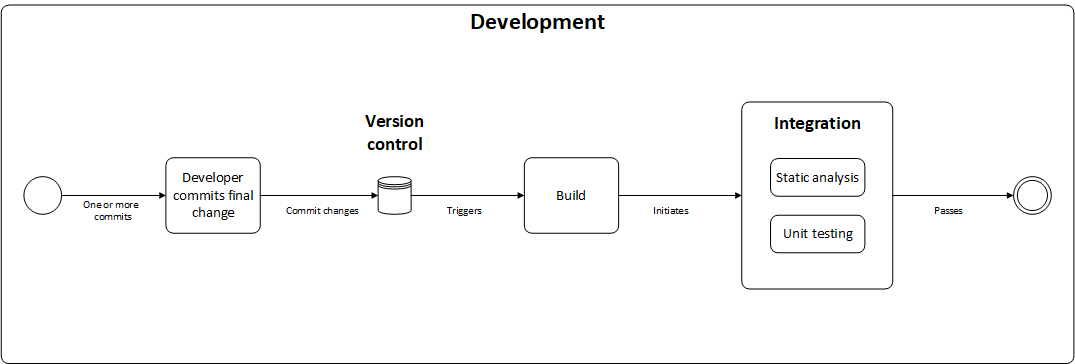
\includegraphics[width=0.8\linewidth]{Cap2/DevelopmentStage.png}
\caption{\textit{Workflow} de um \textit{job} da fase de \textit{development}}
\label{Fig:Fig3}
\end{figure}

\subsubsection{\textit{Staging Environment}}

\hspace{1cm}Na fase de \textit{staging} (\ref{Fig:Fig100}) é produzida uma imagem da aplicação que depois será colocada no repositório privado de imagens. Depois de lançada e validada a aplicação, são feitos testes de integração e performance, a aplicação é validada pelo \textit{product owner} e -- opcionalmente -- pode ser incluída nesta fase uma análise à qualidade de compressão da imagem através da utilização do \textbf{Dive} \cite{dockerdive}.

\begin{figure}[hbt!]
\centering
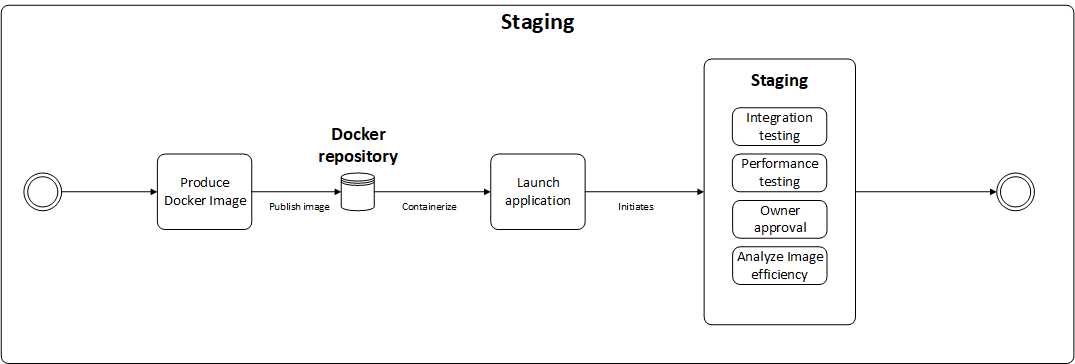
\includegraphics[width=0.8\linewidth]{Cap2/Staging.png}
\caption{\textit{Workflow} de um \textit{job} da fase de \textit{staging}}
\label{Fig:Fig100}
\end{figure}

\hspace{1cm}Faz sentido incluir análise estática nesta fase apesar de não ser obrigatório. A análise estática pode ser utilizada como uma fase extra de verificação ao código da \textbf{Web API} desenvolvida em \textbf{C\#}, uma vez que o código presente em \textbf{VCS} terá de ser validado e aprovado para que o processo de criação da imagem seja automatizado.

\subsubsection{\textit{Pre-live Environment}}

\hspace{1cm}A fase de \textit{pre-live} assemelha-se com um ambiente de produção. O objetivo é precisamente configurar um \textit{job} com um conjuto de processos que simulem a publicação de uma aplicação para produção, juntamente com todos os serviços dos quais a aplicação depende, executar um conjunto de verificações -- nomeadamente validar que o comportamento da aplicação vai de encontro ao esperado -- e submeter a aplicação a uma fase final de aprovação pela mão do \textit{product owner}.

\begin{figure}[hbt!]
\centering
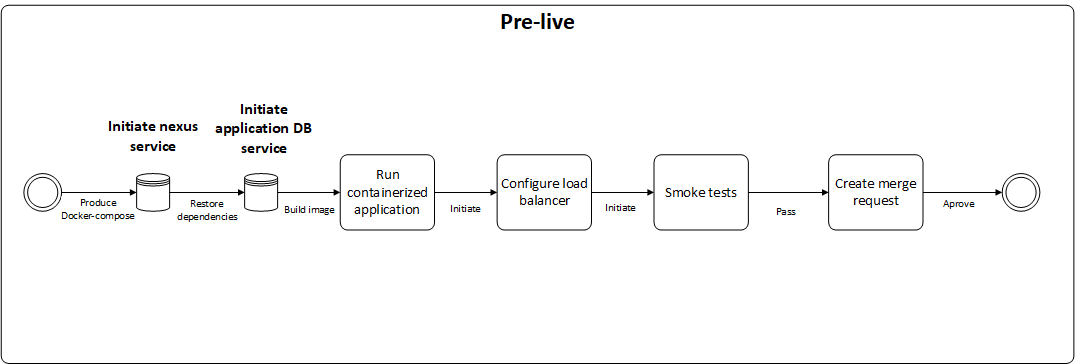
\includegraphics[width=0.8\linewidth]{Cap2/PreLiveStage.png}
\caption{\textit{Workflow} de um \textit{job} da fase de \textit{pre-live}}
\label{Fig:Fig97}
\end{figure}

\hspace{1cm}Como se pode ver pela figura \ref{Fig:Fig97}, a configuração do ambiente começa, à semelhança de uma fase de produção, com a configuração de um documento de composição de todos os serviços (docker-compose.yml) da aplicação. O documento terá de incluir a configuração sequêncial dos serviços por ordem cronológica de acontecimentos, depois são feitos testes à aplicação e opcionalmente pode ser criado um \textit{merge request}.

\subsubsection{\textit{Production Environment}}

\hspace{1cm} A única diferença entre este \textit{job} e o anterior é a remoção dos \textit{tests}, do \textit{merge request} e das validações do \textit{product owner} uma vez que teriam sido feitos anteriormente. Para esta fase pode ser considerada a adição de serviços de monitorização (\ref{Fig:Fig98}) como é o exemplo do \textbf{ELK Stack} (https://www.elastic.co/pt/elk-stack) e do \textbf{Nagios} (https://www.nagios.org/).

\begin{figure}[hbt!]
\centering
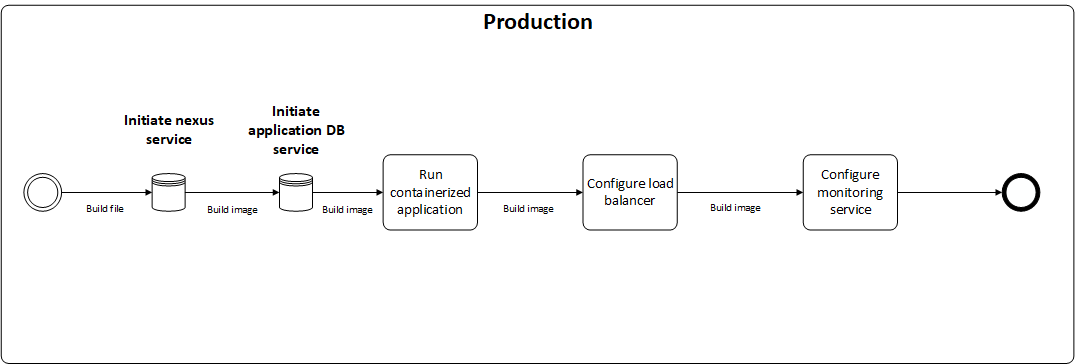
\includegraphics[width=0.8\linewidth]{Cap2/ProductionStage.png}
\caption{\textit{Workflow} de um \textit{job} da fase de \textit{production}}
\label{Fig:Fig98}
\end{figure}

\hspace{1cm}Caso estajamos a considerar a adição destes ou de novos serviços de monitorização na fase de produção é importante ter em mente que todos os serviços devem ser testados e validados previamente durante a fase de \textit{pre-live}. 

\hspace{1cm}É também importante mencionar que estes \textit{jobs}, desenvolvidos para cumprir um conjunto de objetivos pré-estabelecidos num contexto específico, podem não ter o mesmo tipo de resultado quando aplicados a outros contextos de negócio. Ao longo do estágio, durante a construção do protótipo da pipeline, as considerações e as decisões tomadas estiveram de acordo com aquilo que são as necessidades da empresa.